\documentclass[a4paper,oneside,11pt]{report}
\makeatletter
\newcommand*{\rom}[1]{\expandafter\@slowromancap\romannumeral #1@}
\makeatother
\usepackage[margin=1in]{geometry}
\usepackage[doublespacing]{setspace}
\usepackage[citestyle=authoryear]{biblatex}
\usepackage{graphicx}
\addbibresource{references.bib}
\begin{document}
\title{Ascus - Collaboration Finder}
\author{Saad Arif\\Fourth Year Dissertation - First Deliverable \\ \emph{Supervisor}: Ruth Aylett \\ \em \emph{Second Reader}: Patricia Vargas}
\maketitle
\pagestyle{empty} %get rid of header/footer for toc page
\tableofcontents %put toc in
\addtocontents{toc}{\protect\thispagestyle{empty}}
\listoffigures
\addtocontents{lof}{\protect\thispagestyle{empty}}
\pagestyle{plain} % put headers/footers back on
\listoftables
\addtocontents{lot}{\protect\thispagestyle{empty}}
\cleardoublepage %start new page
\pagestyle{plain} % put headers/footers back on
\setcounter{page}{1} %reset the page counter

\chapter{Introduction}
ASCUS(Art Science Collaborative) is a non profit volunteer organisation that is made up of a network of artists and scientists who are looking for interdisciplinary collaboration. ASCUS aim is to advocate and facilitate improved art science collaboration, science communication\autocite{ascus}. However ASCUS does not have any tools  to meet such aims. Currently ASCUS has a single static site which provides information on past events as well as information on the organisation. This site allows users , who wish to participate in collaboration to get initial ideas about the organisation and how to get involved. However the site does not actually help find potential collaboration opportunities. Thus in order to advocate and facilitate collaboration it must be possible for members of ASCUS to have a central location where they can easily and quickly find collaboration opportunities. This project will focus on implementing a application that will allow ASCUS to meet its aims of art and science collaboration.
\section{Aims and Objectives}
The aim of this project is to develop a web application in order to allow artist and scientist to find collaboration opportunities.
The main objectives of the new application are:
\begin{itemize}
	\item Develop a web application that will reduce work load on artist and scientist when looking for collaboration opportunities.
	\item Develop facilities that allow artist and scientists to discuss ideas for collaborations.
	\item The design of the application must allow both artist and scientists to make effective use of it.
\end{itemize}
	
\chapter{Literature Review}
This section will cover the background literature consulted for this project. The literature that was consulted was focused on Expert locator systems. 

Expert locator systems allow users to find experts in a particular area.
This project is focused on building a subset of an expert locator system, that is focused on facilitating the ability to find collaboration opportunities. Thus before building the system , the areas that will be looked at are why do would or would not use an expert locator systems and different approaches to building an expert locators systems,
\section{Organisational need for Expert locator}
Many organisations have identified the need to locate knowledgeable individuals within there organisations. It is important for organisations to effectively use there knowledge in order to enable organisational learning, providing better technical assistance and creating teams to deal with critical situations among other goals\autocite{ackerman2003sharing}. Furthermore an organisation may end up "reinventing the wheel" even though a solution had already been made for a similar problem before. Thus it becomes necessary to catalogue skills and expertise of individuals, who knows what,  in way that it can later be queried\autocite{fernandez2000}.

Examples of organisations developing expert finding systems: \\
Hewlett Packard (HP), a company in the computers and electronic equipment market developed  an Expert-Finder. The goal of the project was to build a network of experts which consisted of a database user profiles. The user profiles gave a summary of the users knowledge and skill\autocite{fernandez2000}.
 
The National Security Agency (NSA) has also attempted to build a system to locate experts with in the organisations. The goal of the his project was similar to HP, identification and cataloguing of knowledge and skills with in the organisation\autocite{fernandez2000}.

ASCUS has similar needs to the previous companies named. The organisation requires a tool that allows its members to find collaborators. Thus it needs to catalogue its members' expertise, so they can be mined by members who are looking for collaborators. 
	
\section{Why do individuals want to seek experts?}
Yimam-Seid and Kobsa(\citeyear{kobsaseid2003}) offer a few reasons as to why individuals may seek experts They state there are two major reasons why individuals seek experts. (a) They need specific information from the expert and (b) They need the expert who to perform some function. The people seeking experts for the first reasons are usually looking to replace or complement other sources of information such as documents. Some scenarios for this reason include seeking information that is not documented, using experts to minimize ones own effort or individuals may prefer interacting with humans rather than documents or computers. 

People seeking experts for the second reasons need experts for a continued period of time where the expert will be working for them or with them. Usually the search for this type of reason is performed more carefully than for obtaining information from experts.

ASCUS members looking for collaboration fall into both categories. While members may be be looking for active collaborators to participate with in their project, they may also be seeking advice or information into a field they have no expertise in. Thus it is important for the system to facilitate both types of members.

\subsection{Why people do not want to seek experts?}
Allen (\citeyear{allen1977}) noted some reasons as to why information seekers may not want to use their colleagues as a source of information but rather would rather use other information channels. In his study of 19 engineers, he found a higher correlation between frequency of use accessibility than quality of the source of information. He further found that information seekers, found the transaction of information seeking as a costly one. The the cost was perceived in the chance of a response that maybe "ego threatening", a loss in status and seeming incompetent. For these reasons engineers would first look at documentation as a source of information. T

While it has been shown there are issues when seeking experts, they are not of primary concern. ASCUS is organisation for collaboration thus it is assumed that members are looking for interaction. Further it can be assumed that many members have already been part of collaborations and thus the previously stated issues should not apply to these members.
\subsection{Stages of finding Expertise}	
\citeauthor{mcdonalackerman1998}(\citeyear{mcdonalackerman1998}) identify three stages individuals went through to find expertise with in an organisation, Expertise Identification, Expertise Selection and Escalation.  
\subsubsection{Expertise Identification} 
Expert identification is defined as \enquote {the problem of knowing what information or special skills other individuals have.} It is further noted that expertise identification is difficult problem to solve.It contains many varying factors such as what is expertise , how will it be used within the given context and the problem of handling the change of individuals skills and expertise as time goes on. One solution to such expertise identification is to \enquote {consider the types of historical artifacts that are employed by local users as resources and then incorporate use of those within the system.}\autocite{mcdonalackerman1998}
\subsubsection{Expertise Selection} 
After determining who has what expertise it is intuitive to then select the most appropriate individual(s) that will solve the problem \citeauthor{mcdonalackerman1998}. (\citeyear{mcdonalackerman1998}) define expertise selection as \enquote {appropriately choosing among people with the required expertise.} Furthermore they observed that expert seekers usually used three expertise selection criteria, \enquote {organizational criteria, load on the source and performance.} Expert seekers tried to find experts that were local and when that failed they went to different departments within the organisations. Expert seekers, further more took into account how busy experts were, approaching the least busy first. Finally they firstly approached experts that were better at explaining solutions or had better \enquote {attitudes}.

\subsubsection{Expertise Escalation} 
Escalation is the process by which people resolve the failure of the expertise identification or selection mechanism. The expertise seeker may try to identify other experts or pursue other experts that maybe able to solve the problem.  This does not necessary involve asking members higher up in the organisation hierarchy, it may involve asking help from less desirable experts or even searching for experts in a different department within the organisation\autocite{mcdonalackerman1998}.

The system being built should emulate the first two stages and try to avoid the third stage as much as possible. The system ,with regards to expertise identification, should try to match with as much accuracy as possible if a person is an expert in a particular area. In the second stage the system should order the found candidates in an ranked list with the top candidate the most useful to expert seeker. The ideal solution would be to never reach the expertise escalation stage at all but their is no known system that is 100\% accurate in expertise identification and selection. Furthermore it is unclear from the literature as to how a system can help the user in the expertise escalation stage.

\subsection{Traditional Approach}
Many organisations contain roles which act as expertise or information locators.
In Allen's(\citeyear{allen1977}) discussion he presented a highly linked role within an organisation , which served to bring relevant information to informations seekers. Other researchers have have found similar roles within different types of organisations. \citeauthor{ehrlichcash1994}(\citeyear{ehrlichcash1994}) found a what they called an \enquote{information mediator}, who because of his breadth of knowledge and interpretation skills was the go to person in case of any problems. They also noted that the information mediator was a critical part of the organisation. \citeauthor{mcdonalackerman1998}(\citeyear{mcdonalackerman1998}) found role that they called \enquote{expertise concierge}. The expertise concierge has the knowledge of who within the organisations knows what. When a person who is looking for expertise , they ask the expertise concierge about people who maybe be able to help then the concierge will use their knowledge to suggest individuals that match the query.

One way in which we can emulate and automate such roles is by building an expert database. Such an idea works by manually entering expertise data into the database, which can then be queried. The expert database will return a set of individuals that may be of help. Furthermore the expert database  may return the individuals in a ranked list such that higher up the list individuals are, more likely they are to be of help. However such a system do have limitations\autocite{kobsaseid2003}.
\begin{enumerate}
	\item Developing the databases is a labour intensive and expensive.
	\item For the such a system to work , it relies on the experts willingness to spend time 		  			  initially providing information about their expertise.
	\item Due to a continuous change in peoples expertise it is hard to keep the databases up to 				  date.
	\item There is usually a disconnect between expertise description entered into the database and 	          the expert related query. The expertise description are usually general and incomplete                                                                            		  while the expert related queries are very specific. 
\end{enumerate}

\subsection{Contemporary Approach}
In order to combat the limitations of the traditional approach the expert finding process is further automated. This is done by automatically obtaining information on experts from many different sources and not relying solely on human sources\autocite{kobsaseid2003}. Using this method the experts do not need to update their profile manually and thus it is always up to date. 

However this approach has many difficulties. Firstly it is can be difficult to find sources on which to judge the skill level of an expert in a particular area. An example source for scientist could be articles published but for artists this much more difficult as their work is more difficult to analyse. A common interdisciplinary source that can be used to within an organisation, are email communications. Emails can demonstrate expertise, as queries can be answered by the expert and communication patterns can help determine who has what knowledge with in the organisation\autocite{campbell2003}. However using such a source requires handling privacy concerns. 
Even with a source of information it still difficult to determine the weight of the source. for example if a scientist co authors an article does that make the scientist an expert in that area? did both authors equally contribute to the article?. Such questions are difficult to answer without further information and if sources are not properly weighted then it is more likely for incorrect experts to be identified.


%should be simple

%projects people can search.
%project page has title, description, goals, looking for who, comment section, links of people profile currently in the team
\chapter{Requirements}
The requirements of the project are prioritised in order to manage the project effectively. The most important requirements are given the tag High. These requirements must be completed before the end of the project. The next priority tag is Medium, any priorities with the Medium tag will be started only after the High tag requirements have been finished. While the Medium tag priorities are not essential, it is recommended that at least some of them be part of the system if not all. Finally the least important requirements will be given the tag Low. These requirements are not needed for the main functionality and only provide extra features for convenience .

\subsection{High Priority}
\subsubsection{Search for Collaborators} 
This is has been identified as the most important requirement. The users shall be able to search for collaborators in the database. The criteria for search shall be:
\begin{description}
	\item[Area of work] The user must be able to search for collaborators in the database who are Artist or Scientists.
	\item[Location] Search for collaborators in a particular city.
	\item[Distance from user] Search for collaborators with in a certain distance from the city the user is in. The user will not need to register to use this functionality.
\end{description}
	
\subsubsection{Register and Log in} 
 User shall be able to register as member and customize their profile. To register the user must provide a first and last name as well choose a user name and password. Once the user has registered they can then customize their profile. The profile shall contain the following items:
 \begin{itemize}
 \item first and last name (Required)
 \item age (optional)
 \item email (optional)
 \item Phone/Mobile number (optional)
 \item Biography (optional)
 \item Artistic and/or Scientific interest (optional)
 \item Profile Picture (optional)
 \item Extra pictures - in order to demonstrate some previous work (optional)
 \item External Links - in order to show previous work done, such as blogs and journal articles (optional)
 \end{itemize}
 The username and password provided will be used to login, which will allow the members to edit their profile.
 	Members can only edit their own profiles. While only administrators can remove members, which in turn will also remove the profile.

\subsubsection{High usability} 
This as been given a high priority as an application with high usability and consistent design will attract more users. Even with a functional application in order to for the application to be successful and help collaboration, the user must find it intuitive and easy to use.
\subsection{Medium Priority}
\subsubsection{Map visualization}
This feature allows users to visually see the location of members in a map. The map will show user dots representing members on map. The dots will become bigger as more members are in a particular area. There should be a zoom functionality, as the user zooms in the more detailed density of the members becomes clear. This is likely to be the most difficult requirement and is likely to scoped down in order to be manageable with in the project deadlines.
\subsubsection{Projects}
This feature will allow members to create projects, that users can search for. The project should have a Title, description,images to demonstrate ideas, goals and what skills are required. The original member to start the project can edit the project and delete the project. There will be a comment section for each project allowing members to give feedback and ask questions. Administrator can only delete the project.
\subsection{Low Priority}
\subsubsection{Forum}
User will have the standard forum functionality available . Users will be able to create threads and post comments. 

\chapter{Technology Analysis}
\section{Database}
The database will be used to store user details such as log in and password as well as the users information displayed on the users profile.
\subsection{MySQL}
MySQL server is open source relational database with extensive customisation options for performance tuning. It also offers capabilities to set user accounts and permissions. The author has experience in working with MYSQl.
\subsection{SQLite}
SQLite is a relational database in the public domain. Unlike the other databases servers mentioned, this software does not operate in a client-server model,the database is contained within a file. Thus the SQLite databases can be embedded into an application while other databases works by having a separate database server with which to communicate.
\subsection{Conclusion}
Both database have similar features and both perform slightly different tasks. MySQL offers more control, while SQLite offers easy of set up. Due to the short time in which this project will take place, the MySQL database is chosen as the author has previous experience in it, allowing for immidiate productivity.

\section{Server Side} 
\subsection{Ruby on Rails (RoR)}  
Ruby on Rails is a framework built on ruby programming languages and uses a MVC arhictecture. The RoR philosophy is convention over configuration. By following the set of conventions the developer can be more productive and the framework "just works". Thus it is possible to be very productive but it does have a steep learning curve. Further it is relatively new, being created in 2005, it lacks the mature documentation of `.

\subsection{Active Server Pages (ASP)} 
 Active Server Pages (ASP) is a web framework from Microsoft, that you can use to create and run dynamic web applications\autocite{microsoftasp}. In order to use ASP a the server must run a Microsoft I.I.S. (Internet Information Server) operating system.Further more the database must be Microsoft SQL Server(MS-SQL). Though it is only limited to the windows platform, without considering third party tools allow for cross platform functionality, it does integrate well with other windows technologies.
 
\subsection{PHP Hypertext Processor (PHP) } 
PHP is a general purpose language suited for web development. It provides many features suited for web development and can be used as scripting language. PHP is one of the most widely used programming languages for the web, thus has mature documentation as well as plethora of tools to support its development. It also considered to the have lowest barrier to entry as it is very easy to set up. Furthermore the author has previous experience in PHP.

\subsection{Conclusion}
PHP will be used for server side scripting, as it is mature and well documented. Furthermore the previous experience allows the author to be productive sooner than with other technologies.
\section{Testing}
In order to preform thorough testing it is important to automate the testing by using a testing framework. By automating it becomes easy to perform tests after every change to the application and any issues will be immediately reported. From this, it saves the developer from wasting time manually running algorithms on data.Furthermore Automated tests can easily execute many of different types of test cases during every test run providing a wide coverage which is difficult to do manual tests.

For PHP two popular unit testing frameworks will be considered, PHPUnit and SimpleTest. Both testing frameworks provide similar features such as creating unit tests , running them automatically and showing failed tests and passed test. Therefore evaluating the frameworks will focus on other aspects such as documentations, integration with other tools.
\subsection{PHPunit}
PHPUnit is the standard unit testing framework that is included in many PHP framkeworks such as Zend Framework, Cake PHP. PHPUnit is well maintained as   updates have been done regularly. PHPUnit seems to have larger user base as well as more online tutorials. PHPUnit is integrated into many PHP IDEs  such as Eclipse, Netbeans, Zend Studie, PHPStorm. PHPUnit requires a terminal inorder to run tests.
\subsection{SimpleTest}
SimpleTest is another unit testing framework with the focus on simplicity. SimpleTest is not well maintained with last update over a year ago. SimpleTest does offer the ability to run tests in a web browser thus not needing a terminal, which can be useful when working on a remote web server.Furthermore adding SimpleTest to a project is easy as simply using the include command in a PHP script. While many tutorials are available for SimplTest, many of them are over a year  old. Eclipse IDE offers a SimpleTest plugin.

\subsection{Conclusion}
While SimpleTest and PHPUnit offer similar in features in terms of creating tests and automatically running them, PHPUnit is better maintained thus easier to find documentations and help with issues should any arise. 


\chapter{Risks Assessment}
 	This section will give an an overview of the potential risks to project development.
\begin{center}
	\begin{table}[!ht]
    \begin{tabular}[ht]{| l | l | l | p{5cm} |}
    \hline
    Risk & Probability & Severity & Mitigation Strategy \\ 
    \hline
    Browser compatibility issues & High & Moderate & Constantly test browser compatibility through out the development cycle.Leverage automatic test frameworks in order to supplement manual testing.\\ \hline
    Fall behind on plan & Moderate & Moderate & Give small leeway time for each part of the application. If significantly behind schedule then only complete vital parts of the application.  \\ \hline
    Person of interest is unavailable & Moderate & Moderate &  Another client is kept up to date with the main development of the application.\\ 
    \hline
Users find the system unusable & Moderate & High & Follow user centred design approach. Maintain regular meetings with the client. User testing must be carried out extensively and feedback should be integrated into the next iteration. \\ 
    \hline
    Low quality feedback & Low & Moderate & Pilot all methods used to gain user feedback. If low quality feedback is given reassess previous methods for weaknesses and integrated any findings into a new- questionnaire. \\ 
    \hline
    
    \end{tabular}
    \caption{Risk Assessment}
\label{tab:xyz}
    \end{table}
    \end{center}
\chapter{Methodology}
Due the user centric nature of the of project, it is best to use iterative development and avoid the traditional waterfall methodology. The waterfall methodology is not suited for this project as it does not involve users as much as required for high user interaction projects. 

Using iterative development, this project will focus on cycles of prototyping small parts of the project, implementing the prototype and finally getting feedback. The original prototype will be continually improved as more feedback is obtained.

By using iterative development , the unpredictable nature of working users can be managed. Due to continually prototyping and implementation small parts, the user will still have some functionality even if the project cannot be finished. If the waterfall methodology was used and significant difficulties were encountered, it is likely the project would not finish and have no functionality implemented at all. 

Any issues regarding requirements or user interface design can be solved early on in the development process. Using the waterfall method it would too late to go back and make changes to the design, if there were any misunderstandings in the requirements.
In conclusion many of the problems in encountered when developing interactive software can be dealt with using iterative development. 

\chapter{Initial Design}
\section{Initial User Interface Design}
This section will give an overview of the user interface prototypes created so far. There purpose is to get initial feedback on the interface of the main requirements.

\begin{figure}[!ht]
\centering
\includegraphics[width=\textwidth,height=10cm]{../Desktop/search.jpg}
\caption{Search Page}
\end{figure}
This interface design is for allowing users to search for collaborators. The search bars allow the users to search by occupation, location and radius of the location.
Once the search is complete, a grid of member information will appear. Each member that matched the search criteria will have their profile picture, name and the first few words of their biography are shown. The far right hand side shows popular areas in which members have claimed they have expertise in
\\
\\
The second figure shows the interface design for the second main requirement, the profile page. This shows how the profile page will look after the user has entered his/her details.

\begin{figure}[!ht]
\centering
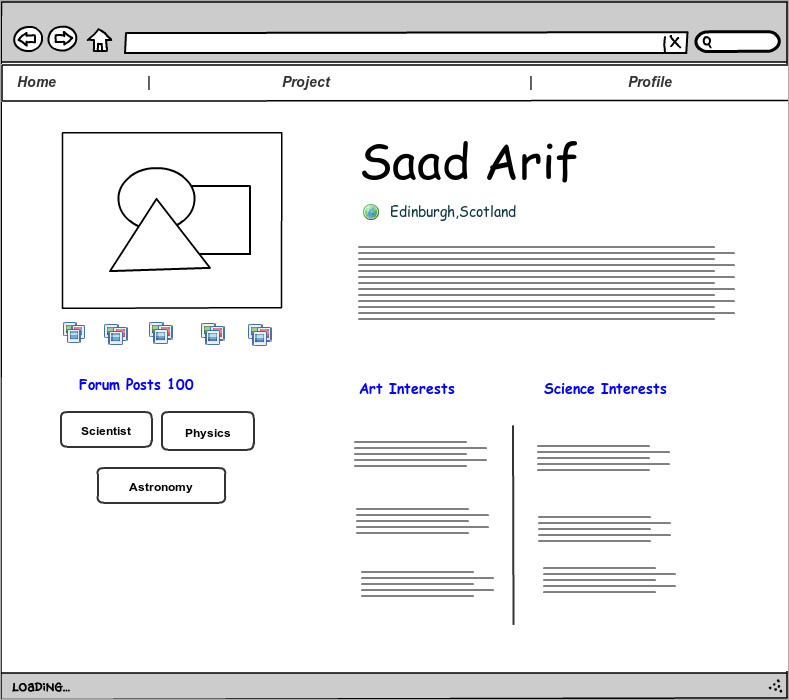
\includegraphics[width=\textwidth,height=10cm]{../Desktop/Profile.jpg}
\caption{Profile Page}
\end{figure}
The profile contains useful information that users are likely to be interested in. It includes location, small biography. Also specific part is dedicated to simply talk about artistic and scientific interests. This will allow for more freedom to say what interests the member regardless of occupation.

On the bottom left it also shows the areas in which the member has claimed to be an expert. Expertise area coupled with the artistic/scientific interest should give the user enough information to judge if the user the is appropriate for collaboration.
\newpage

\section{Initial Database Design}
In order for the database design to reflect the requirements, it is important to identify the separate entities with in the requirements. Three entities were identified, member who has registered, the member's profile and areas of expertise the user has. The figure below shows the relation ship between the entities.

\begin{figure}[!ht]
\centering
\includegraphics[width=\textwidth,height=10cm]{../Desktop/database_diagram.jpg}
\caption{Initial ER-Diagram}
\end{figure}
The relationship between an member and his/her profile is a one-to-one. Each member must have a profile and vice-versa.
\chapter{Initial Testing Strategy and Evaluation}
This chapter describes the plan for testing and evaluating the system.
\section{System Evaluation}
In order to meet the high usability requirement, it is important to involve users when developing the system and user interface. If the system is not usable then the users will not use the system, rendering the project pointless.

In order to evaluate the system, prototypes will be used. The system evaluation will be conducted by allowing expected system users to interact with the prototypes. Afterwards the user will be asked to fill out an questionnaire, which will include open and closed questions. The closed questions will be used focus on a particular aspect of the design, while open questions will be used to get in depth feedback. 

In order to gain even more feedback a semi structured interview will be used. It will be decided in advance which themes and areas are needed to be explored during the interview. Using a semi structured interview allows for more freedom to discuss various areas and explore areas based on the users answers. The interviews will be recorded, as writing the users answers will likely not capture exactly what the user said. It also frees the interviewer to focus on the users answers rather than with writing them down.

Before any questionnaire and interviews are conducted the user will be given an consent form detailing what will the questionnaire/interview involve, all information gathered will be anonymised, the user can withdraw their participation as they see fit and any recordings will only be kept as long as necessary for the project.
\section{System Testing Strategy}
\chapter{Project Plan}
A high level plan below describes the key tasks to be achieved.
\begin{center}
	\begin{table}[!ht]
    \begin{tabular}[ht]{| l | l | p{11cm} |}
    \hline
    Due Date & Version & Task \\ 
    \hline
    15/10/2013 & R1 & Gather initial requirements.\\ 
    \hline
    01/11/2013 & N/A & Conduct Literature review and research into relevant 												  technologies \\ 
    \hline
    22/11/2013 & Final & Hand in final version of the first deliverable \\ 
    \hline
    03/12/2013 & R2 & Create Questionnaire to gather further requirements. Pilot the 										questionnaire and improve it if needed.\\ 
    \hline
    31/12/2013 & WD1 & Create Website design prototype.\\
    \hline
    31/12/2013 & DD1 & Create initial database design and implementation.\\
    \hline
    31/12/2013 & IMP1 & Create an initial implementation of high priority requirements\\
    \hline
    10/01/2014 & N/A & Gather feedback on initial prototype and implementations. Improve 	                  				   the current system according to feedback.\\
    \hline
     17/01/2014 & WD2 & Create website design prototype for high and medium priority 										  requirements.\\
    \hline
    27/01/2014 & DD2 & Update database design in order to facilitate high and medium 		 								 priorities.\\
    \hline
    07/02/2014 & IMP2 & Implement medium priority requirements and integrate with previous requirements.		\\
    \hline
    17/02/2014 & N/A & Gather feedback and improve system based on feedback.\\
    \hline
    27/02/2014 & Final & Create final website design prototype for high,medium and low priority 			 			 requirements.\\
    \hline
    07/03/2014 & Final & Final update to database design in order to facilitate high,medium and low		 		             priorities.\\
    \hline
    17/03/2014 & Final & Implement low priority requirements and integrate with previous requirements.\\
    \hline
    01/04/2014 & Final & Test the systems, fix any bugs and release the system.\\
    \hline
    \end{tabular}
    \caption{Project Plan}
\label{tab:test}
    \end{table}
    \end{center}

\printbibliography
\end{document}
